
% Asset ID: A21RadiansTikZ-004
% Purpose: Sector diagram supporting l = r theta and A = 1/2 r^2 theta.
\documentclass[tikz,border=8pt]{standalone}
\usetikzlibrary{angles,quotes}
\begin{document}
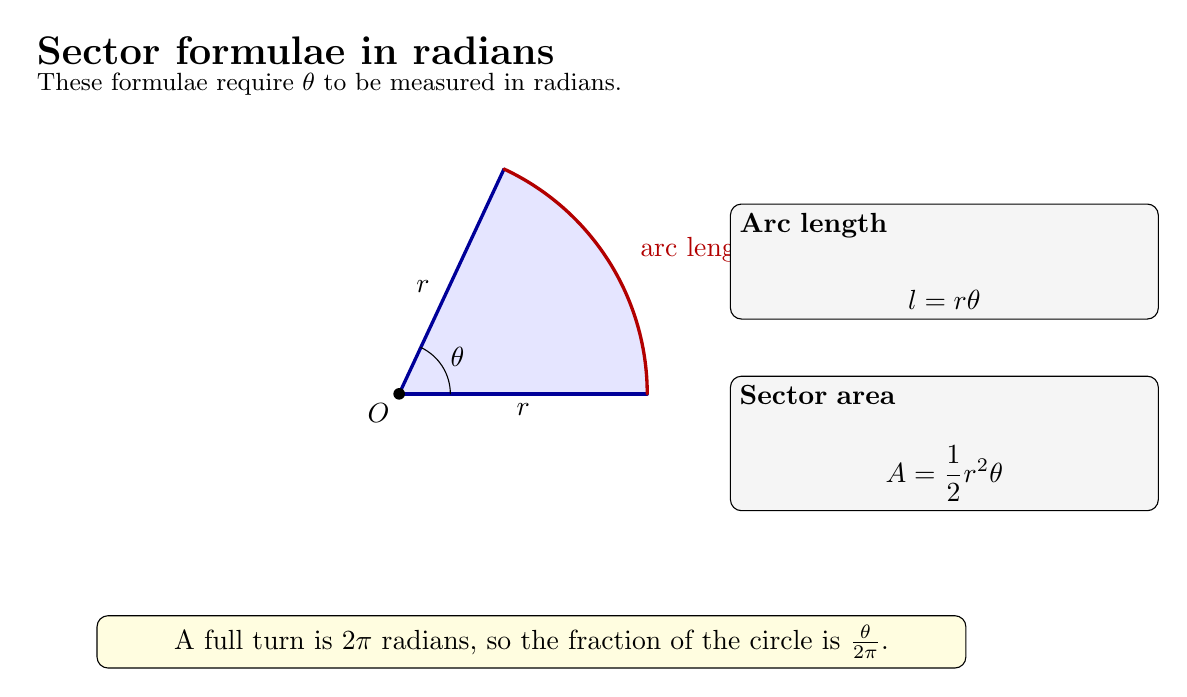
\begin{tikzpicture}[scale=1.05,line cap=round,line join=round]
\def\r{3}\def\ang{65}
\node[anchor=west,font=\bfseries\Large] at (-4.5,4.15) {Sector formulae in radians};
\node[anchor=west,font=\small] at (-4.5,3.75) {These formulae require \(\theta\) to be measured in radians.};
\coordinate (O) at (0,0);\coordinate (A) at (\r,0);\coordinate (B) at ({\r*cos(\ang)},{\r*sin(\ang)});
\fill[blue!10] (O)--(A) arc[start angle=0,end angle=\ang,radius=\r]--cycle;
\draw[blue!60!black,very thick] (O)--(A);\draw[blue!60!black,very thick] (O)--(B);\draw[red!70!black,very thick] (A) arc[start angle=0,end angle=\ang,radius=\r];
\pic[draw=black,angle radius=0.65cm,angle eccentricity=1.35,"\(\theta\)"] {angle=A--O--B};
\fill (O) circle (2pt) node[below left] {\(O\)};\node[below] at (1.5,0) {\(r\)};\node[left] at ({1.15*cos(\ang)},{1.15*sin(\ang)+0.25}) {\(r\)};\node[right,red!70!black] at ({3.3*cos(32)},{3.3*sin(32)}) {arc length \(l\)};
\node[draw,rounded corners,fill=gray!8,anchor=west,align=left,text width=5.2cm] at (4.0,1.6) {\textbf{Arc length}\\[4pt]\[l=r\theta\]};
\node[draw,rounded corners,fill=gray!8,anchor=west,align=left,text width=5.2cm] at (4.0,-0.6) {\textbf{Sector area}\\[4pt]\[A=\frac12r^2\theta\]};
\node[draw,rounded corners,fill=yellow!12,align=center,text width=10.8cm] at (1.6,-3.0) {A full turn is \(2\pi\) radians, so the fraction of the circle is \(\frac{\theta}{2\pi}\).};
\end{tikzpicture}
\end{document}
